%\chapter{PLUME laboratory testing}
\chapter{Basic assessments}
\label{chap:labTests}

  In chapter~\ref{chap:vxd}, an overview of the \gls{PLUME} project was presented.
  Since 2010, the collaboration is building fully functionnal ladders and is trying to reduce the material budget down to $0.35~\%~\rm{X_{0}}$.
  Due to the six sensors working together and the huge amount of electrical lines to control and read the different sensors on a module, the ladders have to be carefully tested and validated in the lab before performing tests under real conditions at CERN or DESY test beam facilities.
  %The chapter~\ref{chap:vxd} has described the \gls{PLUME} project with the different prototypes that were built. 
  %Since the version-1 of \gls{PLUME}, the ladder has a more complicated electrical scheme due to the six sensors on each module.
  %The flex-cable used has a lot of thin metal layers connected to the sensors.
  %The synchronisation, as well the powering and data transmission of the chips have to be work without any problem.
  %%Since the version-1 of \gls{PLUME}, the detector is more complicated due to the six sensors on a module that have to be synchronised and the flex-cable which has a lot of thin metal traces to pilot and read the sensors.
  %Before performing a test under real conditions at test beams CERN or at DESY, the device has to be validated and characterised in the lab.
  This chapter is introducing the different steps from the assembly procedure performed at Strasbourg (for the module) and Bristol (for a complete ladder), to the final tests to study the sensors response, and include electrical functionality tests at Hamburg.
  %This chapter is introducing the different steps from the assembly procedure performed at Strasbourg (for the module) and Bristol (for a complete ladder), to the final tests with a radiation source, and include electrical functionality tests.

  %The \gls{PLUME} ladders are complex detectors and the last prototype was designed to optimise the material budget, by decreasing the width of the flex-cable and the metal traces.
  %Before to perform test in real conditions, the device has to be validated and characterised first in the lab.
  %This chapter is introducing the different steps from the assembly procedure performed at Strasbourg and Bristol, the electrical functionality checks to the tests with a radiation source,

  %Along chapter~\ref{chap:vxd}, the evolution of the \gls{PLUME} ladder design has been presented.
  %The first fully functionnal electrical ladder embeding six sensors on each module was built in 2010 

  %^This chapter is introducing the different steps from the assembly procedure performed at Strasbourg (for the module) and Bristol (for a complete ladder), to the final tests to study the sensors response, and include electrical functionality tests at Hamburg.
  %^Before performing a test under real coniditions at CERN or at DESY test beam facilities, the device has to be validated and characterised in the lab.
 
 \minitoc
  
  %\begin{itemize}
  %  \item Describe bench
  %  \item Describe control of a sensor
  %  \item Describe output of Mi-26
  %\end{itemize}

\section{PLUME assembly procedures}

  The ladders are built in two steps. 
  Firstly, two independent modules are assembled at Strasbourg, then tested at DESY, afterward, they are shipped to Bristol where the modules are glued together on a \gls{SiC} foam to form a \gls{PLUME} ladder.
  The assembly procedures are introduced below, as well as the visual inspection between the mounting steps.

  \subsection{Module and ladder assembly}

    \subsubsection{Module assembly}
    \label{subsec:modAssembly}

    The module assembly is performed at the IPHC by the microelectronics group and is done in three steps.
    First of all, the passive components are soldered onto a flex-cable.
    Then, an epoxy layer with a thickness of $300~\mu\rm{m}$ is applied under the connector side.
    Due to the force applied by pulling and pushing the jumper cable on the ZIF connector, the epoxy layer has the role to reinforce this area and to avoid the flex-cable to be damaged.
    The module is then placed on a metal jig to ensure its flatness using a vacuum suction.
    The next step consists of gluing the six sensors onto the flex.
    The positioning of the chips was used to be done manually, but a programmable robot which has a maximum mismatch alignment reaching approximately $20~\mu\rm{m}$ is now used for this procedure.
    As the sensors are thin and fragile pieces, their are manipulated with a vacuum sucker.
    Few drops of glue are dispensed on the flex and then, the sensors are gently pressed one by one on top of it to be glued.
    Afterward, the glue is cured in an oven and the chips cannot be removed anymore.
    If a sensor is not working properly, it can not be replaced by a new one because the force needed to remove it might break the fragile flex-cable.
    On the worse case scenario, a new sensor can be glued on top of it, but this solution cannot be envisaged for a real ladder as it increases the material budget locally.
    
    In order to avoid this situation, the sensors are probe-tested at the IK in Frankfurt, to select only the good ones before the module assembly.
    The final step consists of soldering the 540 wire-bonds (a single MIMOSA-26 requires 90 wire-bonds) using a semi-automatic machine.
    The wire-bonds can be protected by applying a glob-top epoxy\todo{Citation to a glob-top paper}.
    It has the advantage to offer a protection against moisture or contaminants, an electrically insulation and prohibits their movement during other manipulations (see~\ref{subsec:visualInspection} for the utility of the glob-top epoxy). 
    Nevertheless, it increases the material budget locally and if an electrical problem occurs, the wire-bonds can't be disconnected.
    When the module is assembled, it is finally transferred onto a plastic sole, which has alignment pins.
    This sole helps to manipulate the modules, but also reduces the stress on the flex-cable, by holding it as flat as possible.
    During shipping, a plastic cover is screwed on top of the sole to protect completely the module.
    %Finally, the module is then transferred onto a plastic sole which has alignment pins
    %To test the module, it is transferred onto a plastic sole that has alignment pins.
    %This sole is completed with a plastic cover to protect completely the module during shipping.

    %Control of absolute position about 10 $\mu\text{m}$.
    %Distance between edge of pixel of neighbouring sensors about $500 \mu\text{m}$.
    %Mismatch about $20 \mu\text{m}$.

    %The next step is to sold the wire-bonds (90 for a single Mi26) : semi-automatic machine
    %Modules are then transferred onto a plastic sole for testing and or shipping.

    \subsubsection{Ladder assembly}

    The ladder assembly is performed by the Bristol team.
    It consists of two modules together on a spacer (\gls{SiC}) and a bate (an aluminum plate).
    The operation is done entirely by hands.
    Each module is placed on a separate jig containing grooves and alignment pins to ensure the positioning, as presented on figure~\ref{fig:ladderAssemblyStep1}.
    The sensitive side of the module is facing the jig to have an access to the rear of the flex-cable for the gluing procedure.
    Then, the foam is placed on one module below the sensors, while the bate is glued below the connector with an overlap on the foam (see figure~\ref{fig:ladderAssemblyStep2})
    The second module receives some glue on the backside before the jigs are assembled together.
    The glue is then cured for one day.
    The amount of glue needed for the assembly was studied carefully. 
    Indeed, the surface of the foam is irregular, so if not enough glue is used, the foam will not be glued on the module.
    On the other hand, using too much glue might stick the jigs together.
    When the ladder is finally ready, it is placed into an aluminum box used for shipping but also testing.
   
    \begin{figure}[!h]
      \centering
      \begin{subfigure}[t]{0.4\textwidth}
          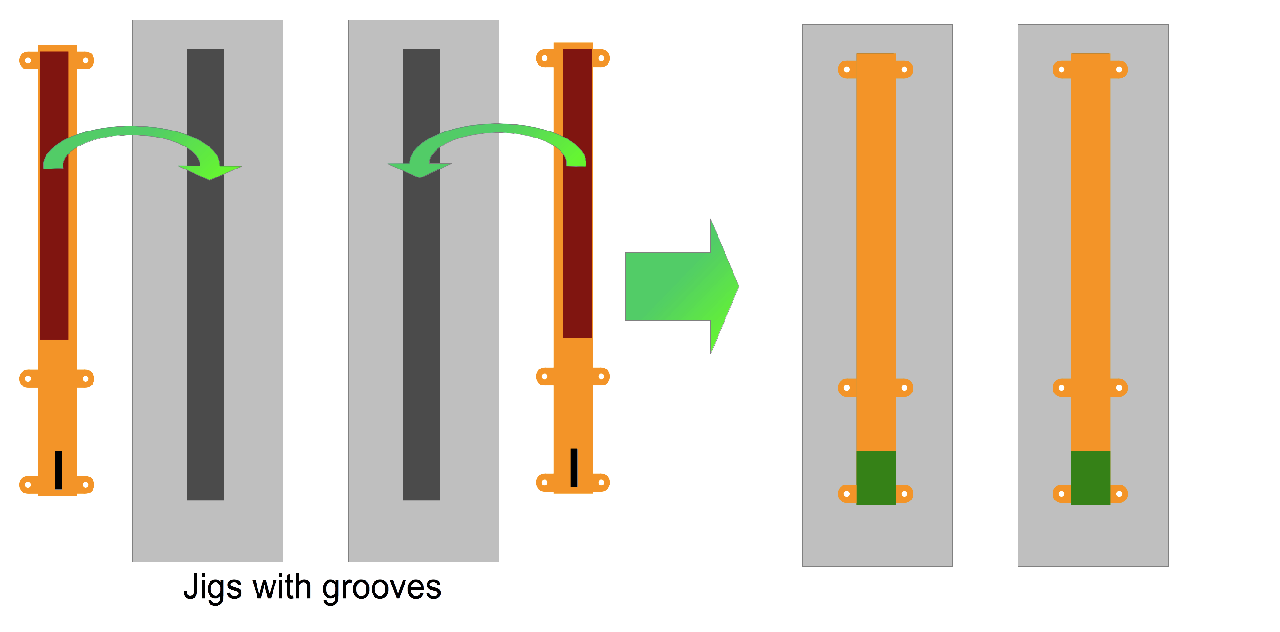
\includegraphics[width = 1.3\textwidth]{Pictures/labTests/plumeLadderAssembly_step1.png}
          \caption{}
          \label{fig:ladderAssemblyStep1}
      \end{subfigure}
      \qquad
       %add desired spacing between images, e. g. ~, \quad, \qquad, \hfill etc. 
        %(or a blank line to force the subfigure onto a new line)
      \begin{subfigure}[t]{0.4\textwidth}
          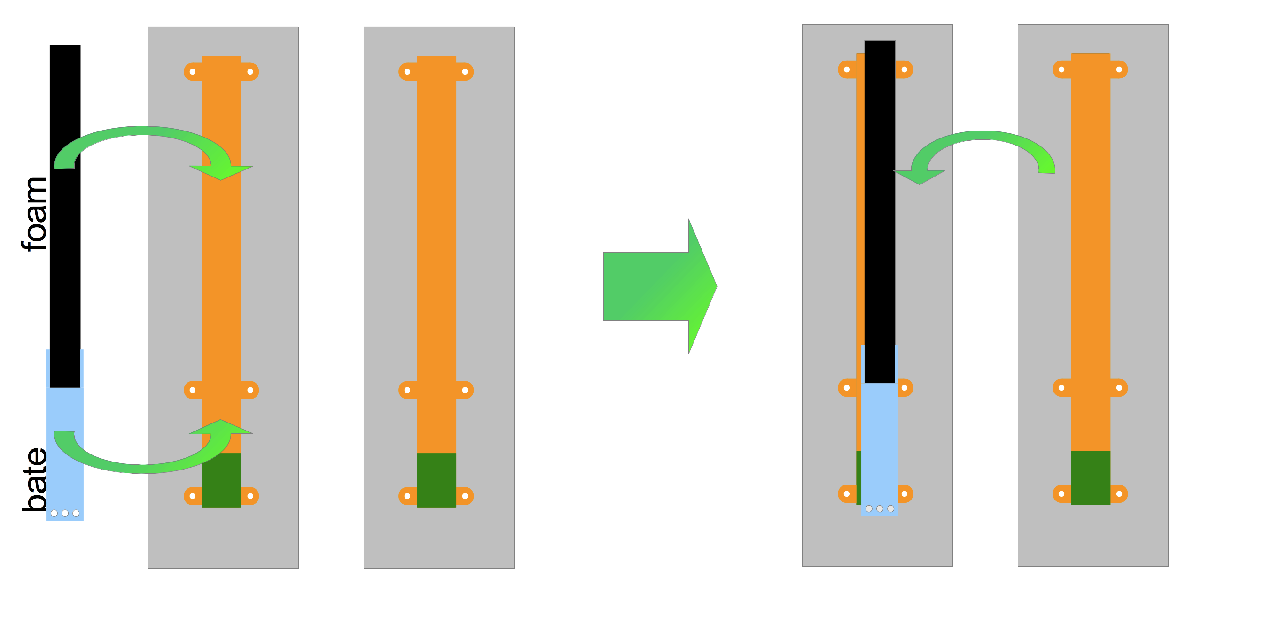
\includegraphics[width = 1.3\textwidth]{Pictures/labTests/plumeLadderAssembly_step2.png}
          \caption{}
          \label{fig:ladderAssemblyStep2}
      \end{subfigure}
      \caption{Drawing of the ladder assembly. The modules are first placed on the jigs, sensors facing the grooves~\ref{fig:ladderAssemblyStep1}, then the foam and the bate are glued between the two modules~\ref{fig:ladderAssemblyStep2}.}
      \label{fig:ladderAssembly}
    \end{figure}    

  \subsection{Visual inspections}
  \label{subsec:visualInspection}

  As explain in subsection~\ref{subsec:modAssembly}, the sensors positioning was performed firstly manually and later was switched to an automatic procedure.
  To tune properly the robot which is in charge of gluing the sensors on the flex-cable, the microelectronic group needs a position feedback.
  The modules are then inspected under a microscope to measure the gap between two sensors, and their position relatively to each other.
  The distance between the last pixel of a sensor to the neighboring one should be less than $500~\mu\rm{m}$, taking into account the $20~\mu\rm{m}$ robot's mismatch.
  The figure~\ref{fig:visAlign} is a picture taken with a microscope showing the relative position of two sensors on the bottom of the matrix for an aluminum straight module.
  %A visual inspection of the position,  as well as any problem on the matrix, as a crack, as well as a check of the wire-bonds have to be done before any electrical validation.
  The gap between the two edges is $\sim 51~\mu\rm{m}$. 
  
  \begin{figure}
    \centering
    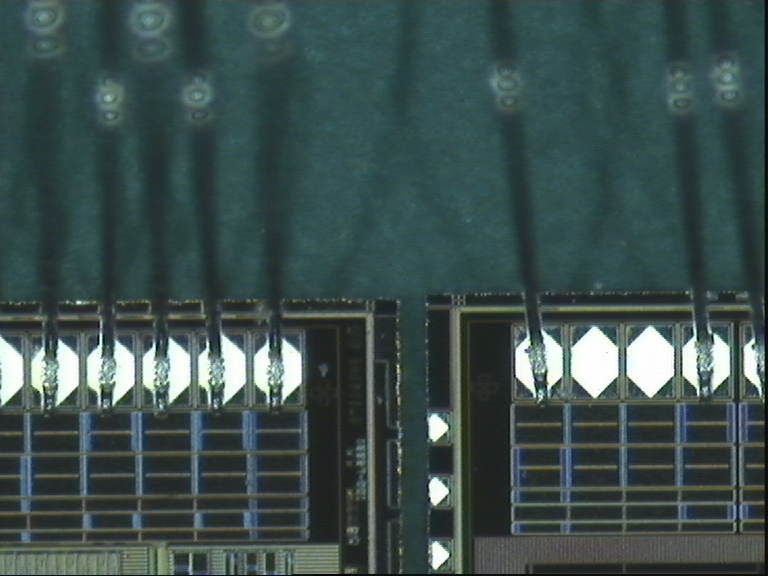
\includegraphics[width=0.6\textwidth]{Pictures/labTests/alignment_sensors.jpg}
    \caption{Visualisation of the alignment. The distance between the two edges is $\sim 51~\mu\rm{m}$.}
    \label{fig:visAlign}
  \end{figure}
  
  The visual inspection is also needed to check if the wire-bonds are correctly connected to the right sensor's pad, to verify that the gluing of the sensors on the flex-cable did not break the matrix due to some dust and also to control that the shipping of the module between the labs (for example between Strasbourg and DESY) did not damage it.
  The modules are fragile objects that have to be manipulated with care.
  Any wrong manipulation can damage severely the vital functionality.
  For example, the figure~\ref{fig:wireBondsCrashed} shows a picture taken with a microscope of wire-bonds crashed due to a falling cable on it.
  The sensitive part and the electronics were not damaged, but some wires were touching leading to a shortcut.
  Fortunately, the microelectronic group at Strasbourg was able to unbend the wires and repair the most damaged one.
  This module is fully operational and working correctly.
  %By using the glob-top method, the wire-bonds can survive to falling cable, but if they are not assigned to the right pad, there is no possibility to correct it anymore.

  \begin{figure}[!h]
    \centering
    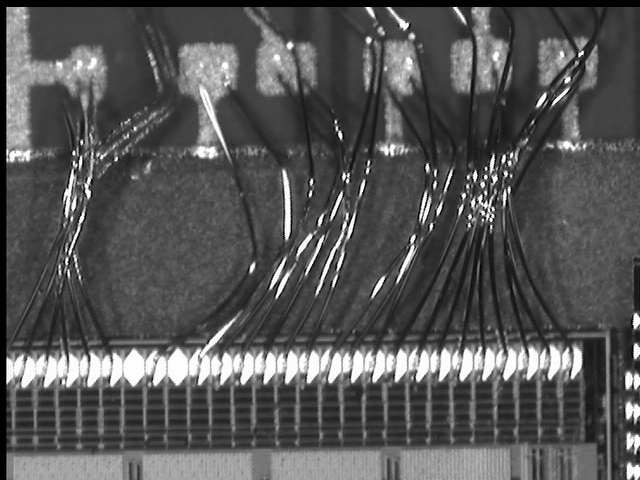
\includegraphics[width=0.6\textwidth]{Pictures/labTests/crash_bonds.jpg}
    \caption{Picture taken with a microscope showing wire-bonds crashed due to a falling cable. Some of the wire-bonds are in contact leading to a shortcut and a non-functional module.}
    \label{fig:wireBondsCrashed}
  \end{figure}

\section{Electrical validation}

  The electrical validation of a \gls{PLUME} module or ladder is performed in two steps.
  The first one consists of checking that all the system controlling and powering the module is working. 
  Then, the module is connected and its consumption, as well as the communication, are checked.

  \subsection{Auxiliary board}

  A module or a PLUME ladder is connected to the outside world by plugging a jumper cable on a ZIF connector at one edge of the module.
  This jumper cable is linked to an auxiliary board which powers the sensors of the module, but also pilots them and to transfer the data to the data acquisition system.
  This auxiliary card is connected to a power supply board which provides the nominal voltages needed by the sensors.
  The power supply board delivers the digital and analog voltages ($V_{DD_D}$ and $V_{DD_A}$ are set to $3.3~\rm{V}$ using two independent potentiometers), the buffers voltage $V_{CC}$ fixed to $3.3~\rm{V}$, as well for the temperature measurement diodes, a $\pm 5~\rm{V}$ for trigger and a power pulsing signal.
  For the lab tests to validate the module, the power pulsing is deactivated by connecting this pin to the $+5~\rm{V}$ pin of the trigger.
  The clamping voltage $V_{clp}$ used for the polarisation of the pixel has to be in the range $\left[2, 2.2\right]~\rm{V}$.
  On the first version of the auxiliary board, it was provided by an external power supply, but the new version delivers the $2.1~\rm{V}$ needed by using an I2C chips or a potentiometer (the user can select which methods to use thanks to a jumper).
  The auxiliary board is also connected to a computer in charge of the sensors' slow control.
  Two RJ45 are providing the \gls{JTAG} registers, as well as the start and reset signal. 
  For a complete ladder, the two modules have to be synchronised and the clock can be injected by a clock distribution board.
  One RJ45 connector is dedicated to the \gls{JTAG} slow control and the signals delivered are: 

  \begin{itemize}
    \item \textbf{Test Data In (TDI)}: received the serial data input feed to the test data registers or instruction register
    \item \textbf{Test Mode Select (TMS)}: controls operation of test logic (for example, by selecting the register)
    \item \textbf{Test Clock (TCK)}: uses to load test mode data from TMS pin and test data on TDI pin at the rising edge, while at the falling edge, it is used to output the test data on the TDO pin.
    \item \textbf{Test Data Out (TDO)}: the output data feed the input data of the next sensor and the last sensor sends the information back to the computer 
  \end{itemize}

  The second RJ45 connector is providing signal coming from the DAQ:
  \begin{itemize}
    \item \textbf{Clock}: has a rate of 80 MHz and is provided by the clock distribution board to synchronise two modules together
    \item \textbf{Start}: signal provided by the DAQ software to start and synchronise multiple sensors (the JTAG start works only for one sensor).
    \item \textbf{Reset}: reset the registers to default value. 
  \end{itemize}

  The principle of the connection between the auxiliary board and the different components to operate one module is depicted on the figure~\ref{fig:plumeAux}.

  Before connecting a PLUME module to the auxiliary board, the voltages have to be set and the \gls{JTAG} communication has to be checked on the auxiliary card.
  Two external power supplies are delivering $8~\rm{V}$ D.C. to the power supply board and are giving an information on the consumption of the whole system.
  The empty auxiliary board has a current consumption about $350~\rm{mA}$.
  Then, the $\text{V}_{CC}$, $\text{V}_{DD_d}$ and $\text{V}_{DD_a}$ should be at 3.3 V, but only the two last voltages can be adjusted thanks to two potentiometers on the power supply board.
  The $\text{V}_{clp}$ is set to $2.1~\rm{V}$ and should not be outside the range $\left[2, 2.2\right]~\rm{V}$.
  The JTAG communication is verified thanks to a probe linked to an oscilloscope.
  The observed signals should be:

  \begin{description}
    \item[TDI:]
    \item[TDO:]
    \item[TMS:] by default is fixed to 1 and change to 0 at every register selection
    \item[TCK:] this clock is slower (30 kHz) than the 80 MHz needed by the sensors and is only dedicated for the slow control
    \item[Reset:] by default is fixed to 1 and should change to 0 every time the reset is called by the JTAG software
    \item[Start:] 
    \item[Clock:] Independently of the method used, the 80 MHz clock has to be correctly distributed along the auxiliary card
  \end{description}

  \begin{figure}[!h]
    \centering
    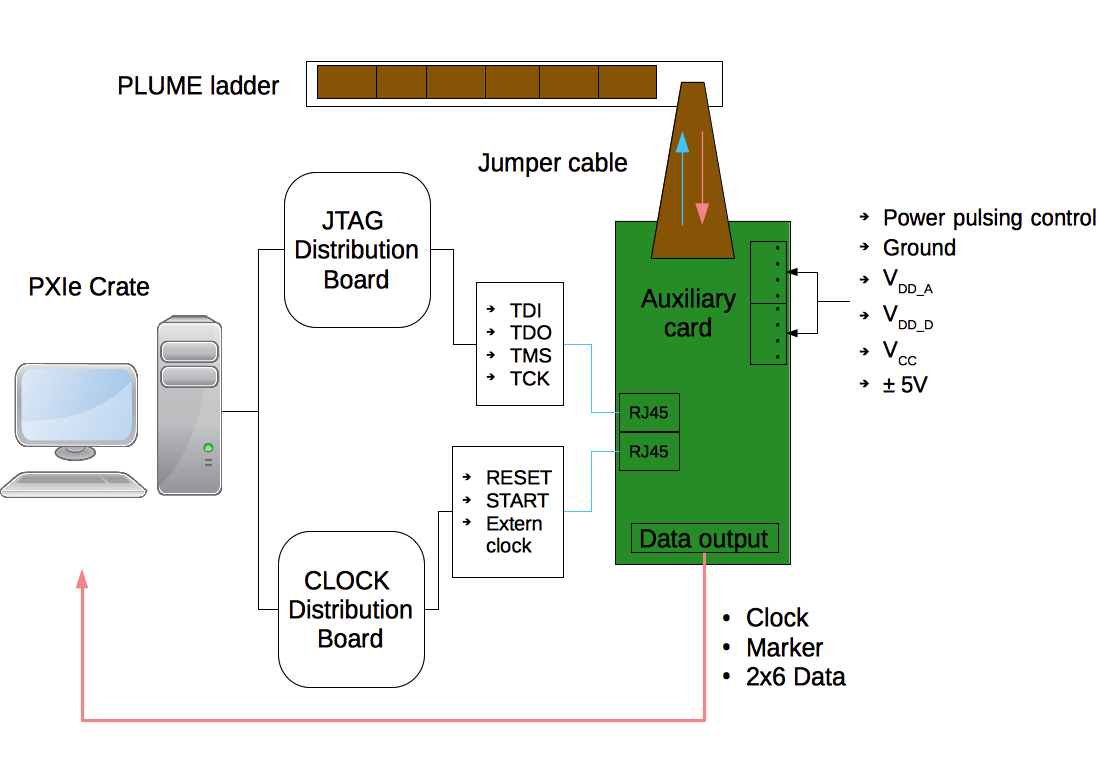
\includegraphics[width=\textwidth]{Pictures/labTests/plumeAux.png}
    \caption{Sketch of the PLUME connection.}
    \label{fig:plumeAux}
  \end{figure}

  \subsection{Smoke test}

  After the validation of the auxiliary board (and the power supplies switched off), the module can be linked to it via a jumper cable.
  The voltages applied to the device have to be adjusted again due to the dissipation inside the flex-cable and the jumper cable.
  The $V_{DD_D}$, $V_{DD_A}$ and $V_{clp}$ can be measured on different pads of the ladder: three pads are closed to the connector, while the three others are at the edge of the flex-cable, as seen on the figure~\ref{fig:voltagePads}

  \begin{figure}[!h]
    \centering
    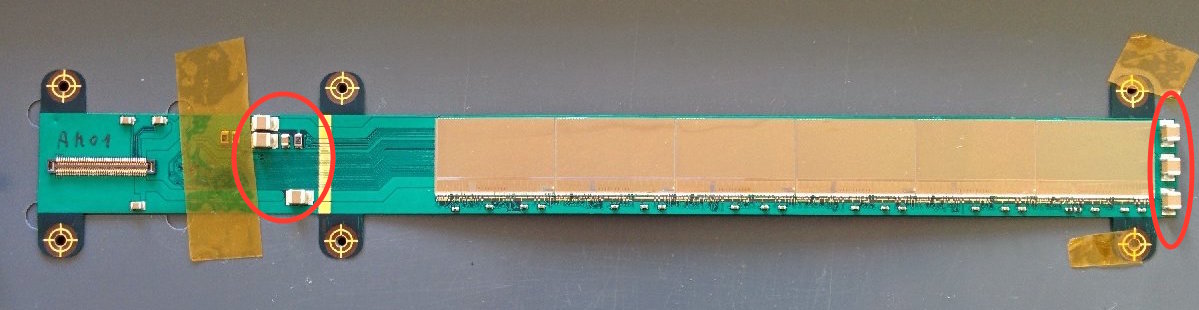
\includegraphics[width=\textwidth]{Pictures/labTests/AM01_voltagePads.jpg}
    \caption{Picture of a aluminum mirrored module with the points of measurement for $V_{DD_D}$, $V_{DD_A}$ and $V_{clp}$.}
    \label{fig:voltagePads}
  \end{figure}

  Two versions of the jumper cable were produced, one very flexible with a high resistivity and the second one stiff with a low resistivity.
 % The first one was not used during the test because of a problem during the fabrication.
  The most flexible cable was not used because of an important voltage drop between the auxiliary board and the module, but also because of a wrong fabrication.
  Indeed, after setting the voltages to the nominal value and plug in the module, a short-circuit happened.
  The auxiliary board tests were correct and were proofed one more time without the module.
  Then, a thermal camera was used to find if a sensor was responsible for the short-circuit.
  One sensor was hotter than the others, nevertheless, the wire-bonds were correctly assigned.
  The problem was coming from a short-circuit between the $V_{DD_D}$ and the $V_{clp}$.
  By passing this two lines on the jumper cable and by connecting them directly to the module, the short was gone.
  Instead of this flexible jumper cable, a stiffer one was used.
  Nonetheless, any movement of the auxiliary board causes a too important stress on the connector and on the flex-cable.
  To avoid any damage, a support was built to hold the auxiliary board and the module on the same frame, thus reducing the risk to break anything.

  The module consumption is checked at every JTAG steps to make sure that no short-circuit occurs.
  Right after powering-on the system, the six sensors are starting in a random state and the consumption at this stage can not point out any electrical problem.
  After the reset of the registers, the total consumption should be around 33 mA.
  Then, the registers are loaded and the consumption should be around 750 mA.
  They are read-back by the JTAG software, which indicates if errors occur.
  If during the reading step no error was discovered, the sensors can be operated and their consumption should be around 1300 mA.

  %Before to present the next step to control the JTAG communication of every sensor, let's introduce the MIMOSA-26 output.

  %\subsection{Mimosa-26 output}

  An inspection of the output with an oscilloscope is performed to check the slow control and to estimate the response of the sensor.
  For the normal mode data format with SUZE enable, the output data of the last frame is sparsified and transmitted during the acquisition of the current one.
  The information provided by the MIMOSA-26 is contained in four output lines.
  The first output line corresponds to the \textit{clock} which is always running even if the data transmission is finished. 
  Its rate depends on the clock rate register. 
  For the normal output mode, it is 80 MHz.
  The second output line is the \textit{marker}, which is available in all mode.
  It is set during four clock's rising edge cycle and might be used to detect the beginning of the data transmission.
  Then, the two last output lines are dedicated to the data.
  They contain multiple information.
  First of all, the beginning and the ending of the data transmission is determined by the \textit{header} and \textit{trailer}.
  They can be used to detect a loss of synchronisation.
  They corresponds to $2 \times 16$ bits (\textit{header0-header1} and \textit{trailer0-trailer1}) and are totally configurable through the JTAG software.
  The \textit{header} is followed by the \textit{frame counter} which corresponds to the number of frames since the chip was reset. 
  The information is separated into two words (\textit{FrameCounter0} corresponding to the least significant bit and \textit{FrameCounter1} corresponding to the most significant bit).
  Then, the \textit{data length} gives the number of 16 bits words of the useful data. 
  The useful data is split into \textit{states/line}, which contains the address of the line which has a hit and an overflow flag if the number of states is bigger than the memory limitation.
  It is followed by the \textit{state} giving the number of consecutive hits and the address of the first column.
  Finally, the \textit{trailer} is ending the data transmission followed by 32 bits of zero.
  The figure~\ref{fig:mi26Output} is a picture of an oscilloscope output of a MIMOSA-26 data output. From the top to the bottom, it shows the 80 MHz \textit{clock}, the four clock's cycle \textit{marker}, the \textit{data0} and \textit{data1} with the \textit{header} and the \textit{frame counter}.
  More information about the MIMOSA-26 can be found in the MIMOSA-26 user manual\cite{manualMi26}.

  \begin{figure}[h]
    \centering
    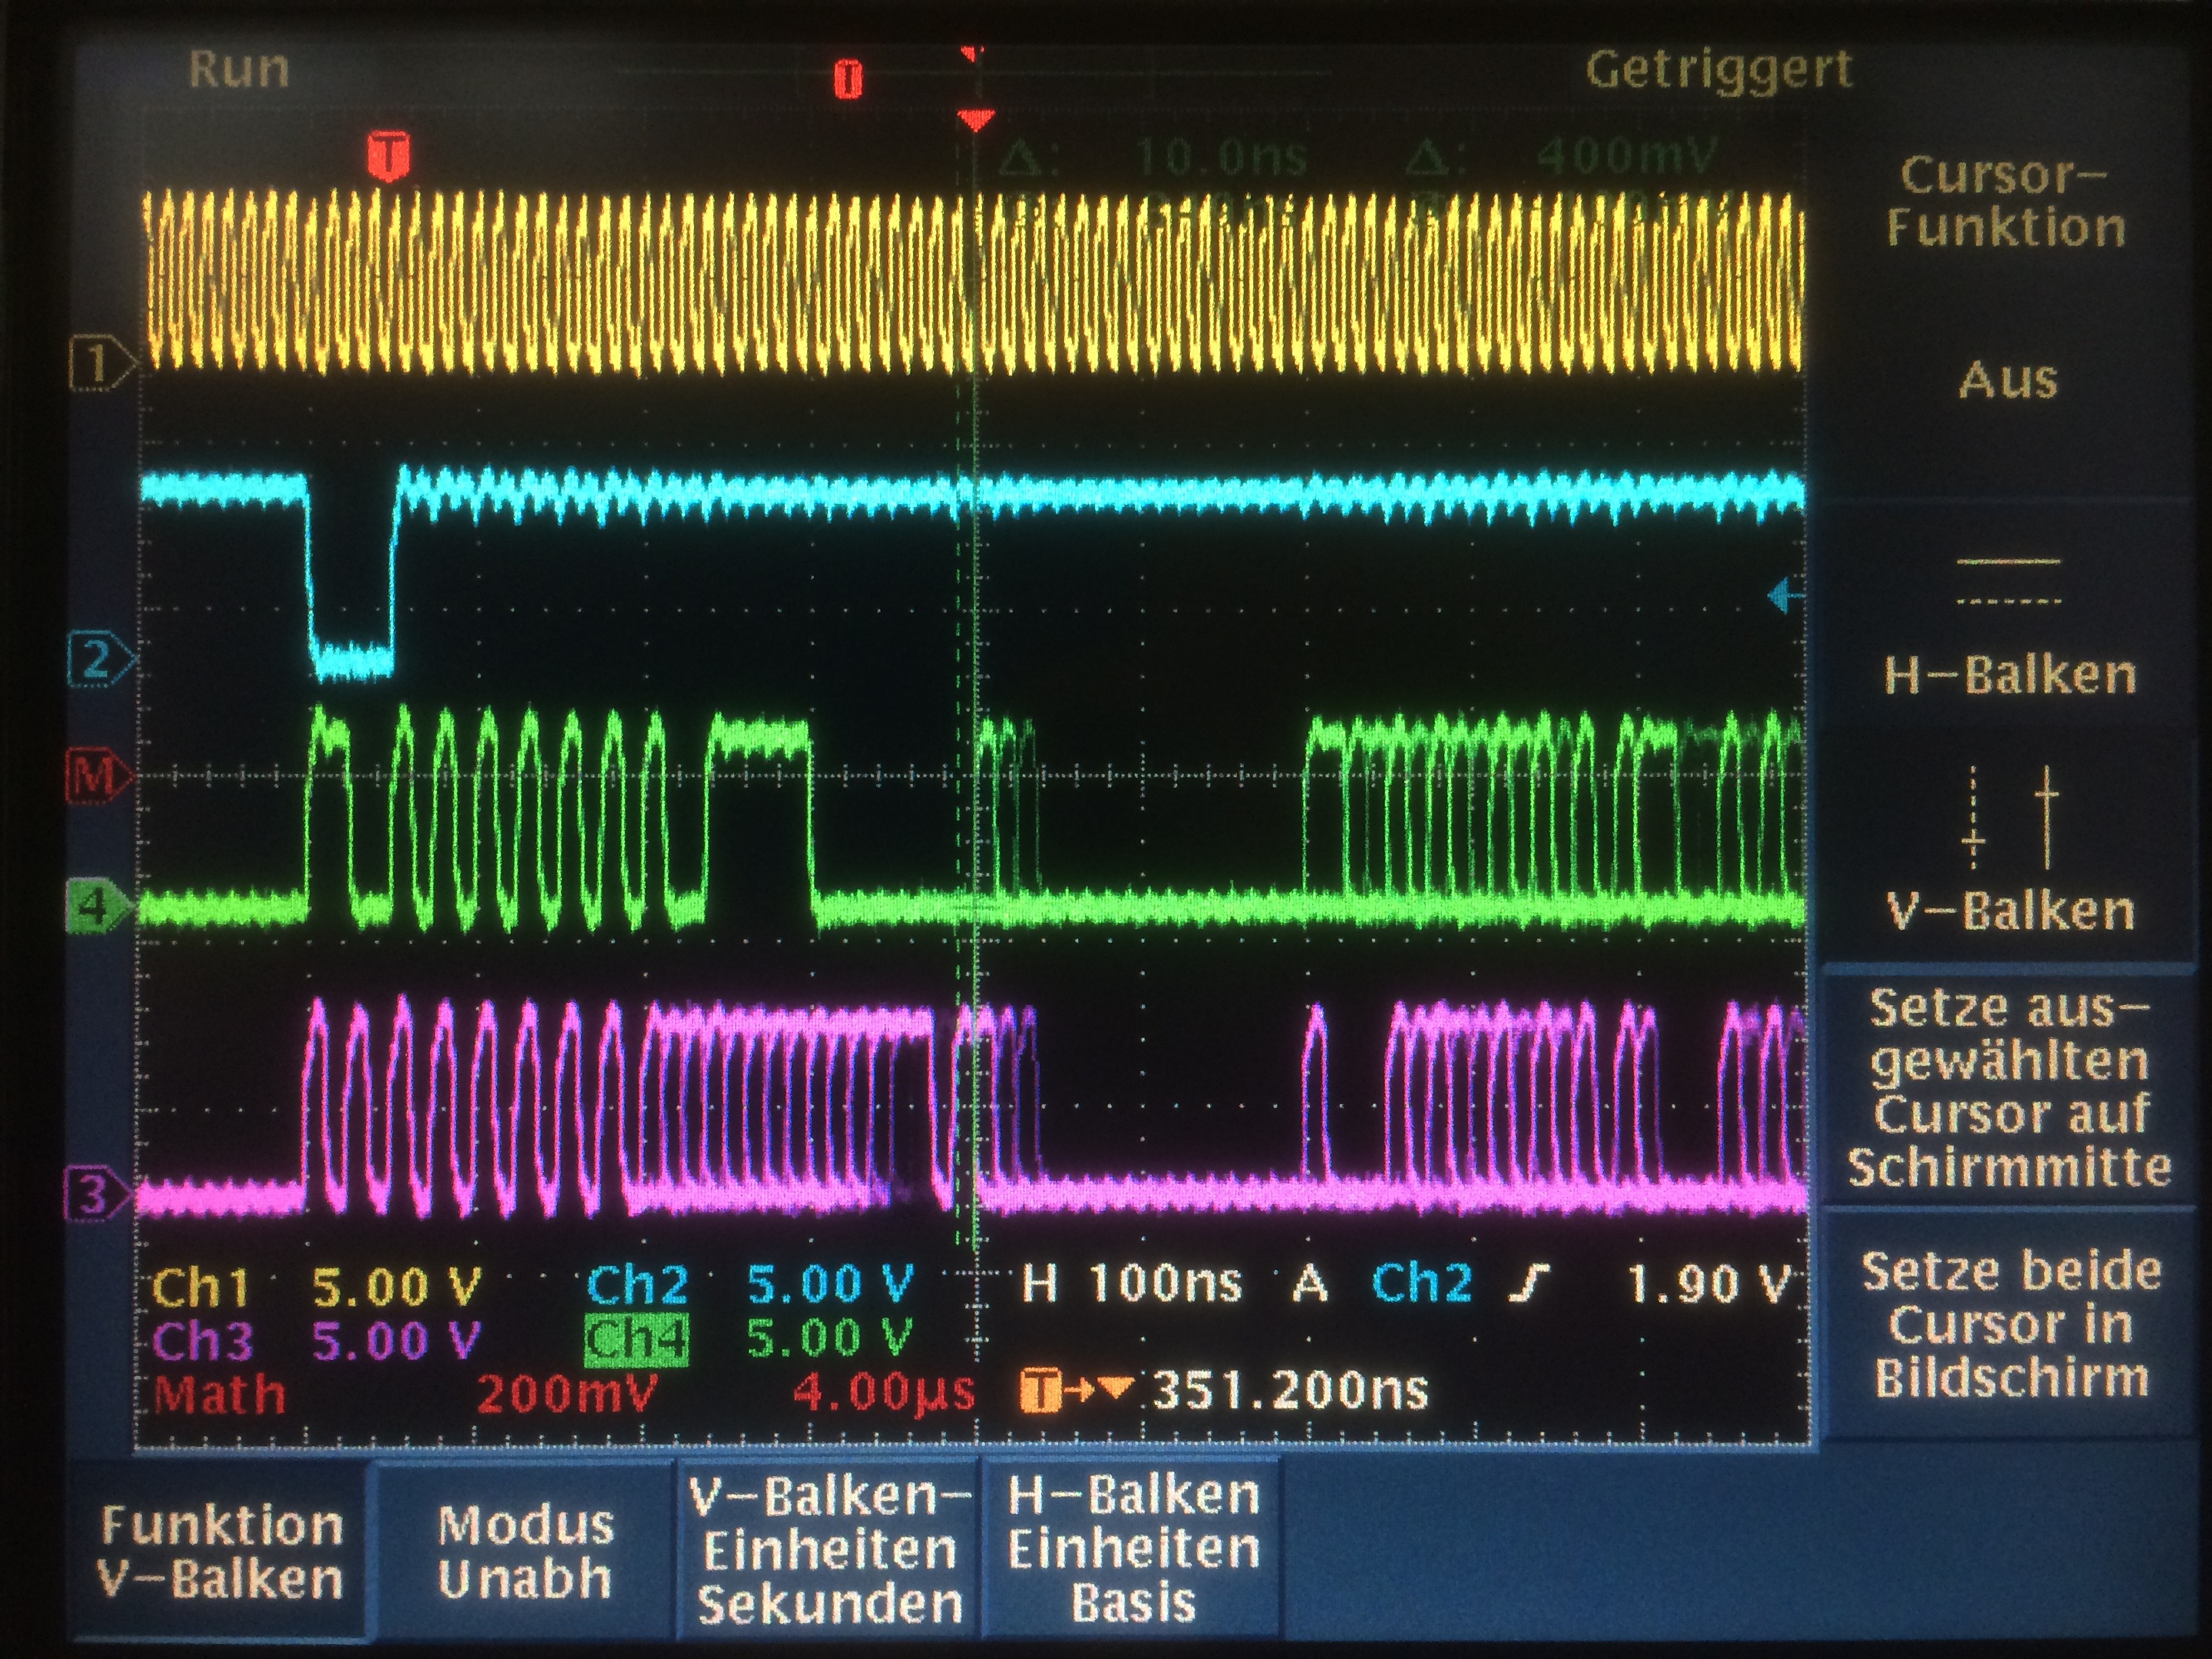
\includegraphics[width=0.8\textwidth]{Pictures/labTests/mi26_output}
    \caption{MIMOSA-26 output from oscilloscope. The top yellow line corresponds to the clock, the blue line below to the marker (which last 4 clock cycles), and the green and purple line are the data output containing the hit information}
    \label{fig:mi26Output}
  \end{figure}

  \subsection{JTAG communication}

  After adjusting the voltages and looking for any short-circuits, the next step is to control the JTAG communication for every sensor.
  As in the PLUME module, all the sensors are synchronised, only the \textit{clock} and \textit{marker} from one sensor is read back.
  On the oscilloscope, the trigger is set on the \textit{marker}.  
  The sensors are configured in the normal mode data format (80 MHz with zero suppression output) and the output is checked in three steps.
  First of all, the sensor is reset, the registers are loaded and read back and then the start signal is sent. 
  Through the JTAG software, the \textit{header} and \textit{trailer} are modified several times and are checked thanks to the oscilloscope.
  Then, the discriminators' response is visualised, specifically to find pixels always sending data even if the discriminators are closed.
  The number of defective pixels and their position is then estimated.
  After that, an estimation of the threshold discriminator values to get few hits are determined and the response is then checked.
  Nevertheless, using light to estimate the response of the sensor can impact the pixels' baseline and modify the normal behavior of the matrix.
  For example, instead of sending more information, the pixels are less responsive.
  Thus, using a radiation source is a better solution.

\section{Noise measurements}
\label{sec:noiseMeasurements}

  In chapter~\ref{chap:vxd}, the principle of the \gls{CMOS} sensors is described and the noise of this technology is discussed.
  As a reminder, the two noise contributions are the \acrfull{TN} and the \acrfull{FPN}.
  The \gls{FPN} is determined as an offset to subtract from the pixel response to reduce its non-uniformity response, while the \gls{TN} is coming from the contribution of different noises during the reset, the integration and the readout of the pixel.
  These noises have to be measured in the lab in order to find the optimum configuration to detect physics signal and reduce the noise impact on the measurement.

  \subsection{Characterisation bench}

  The noise is estimated with a bench of characterisation composed of a National Instrument PXIe crate equipped with a 6562 digital card, two power supplies, a power distribution board, an auxiliary and a JTAG card, as well as the module to test.
  The procedure described here is applied to a single MIMOSA-26, or a PLUME module, as well as an MIMOSA-28 sensor.
  Nevertheless, the data acquisition software used during the characterisation is slightly different to match the clock speed, depending on the sensor technology.
  The four data outputs are connected from the pins on the auxiliary board to the digital card thanks to a National Instrument spider cable.
  Firstly, a test pattern, which loads automatically a \gls{JTAG} file for this test, is done to read the \textit{header} and \textit{trailer} during several frames with a determined data length.
  It has been observed that the \textit{clock} output cable has to be $80~\rm{cm}$ longer than the three other cables to ensure the synchronisation on the rising edge.
  If this is not done or if one of the cables has a wrong polarity, the software is not able to read the \textit{header} and \textit{trailer} and the characterisation can't be done.

  Then, the sensors are configured in the discriminator output mode.
  The zero suppression mode is bypassed, pixels and discriminators are in normal mode ( the whole matrix read in $115~\mu\rm{s}$), but the readout frequency is lower ($10~\rm{MHz}$) via two LVDS output pads.
  The control of the discriminators is divided into four sub-matrices, each containing 288 columns.
  Thus, for one sub-matrix a threshold value in DAC units in the \gls{JTAG} software is driving all the discriminators, depending on a baseline value.
  For one line, usually one located in the middle of the matrix, its baseline response is studied to find the "middle-points" by looking for the threshold of each sub-matrix, in which the discriminators are reaching a half activation.
  When this "middle-points" are determined, the homogeneity of the matrix is checked, as shown on the figure~\ref{fig:homogeneityMi26}.
  Due to the structure of the sensor, the homogeneity is not perfect and some dispersions in the discriminator response are observed between the beginning and the end of a sub-matrix.
  Moreover, to reduce this dispersion, the reference baseline, and the clamping voltage have to be adjusted.
  
  \begin{figure}[!h]
    \centering
    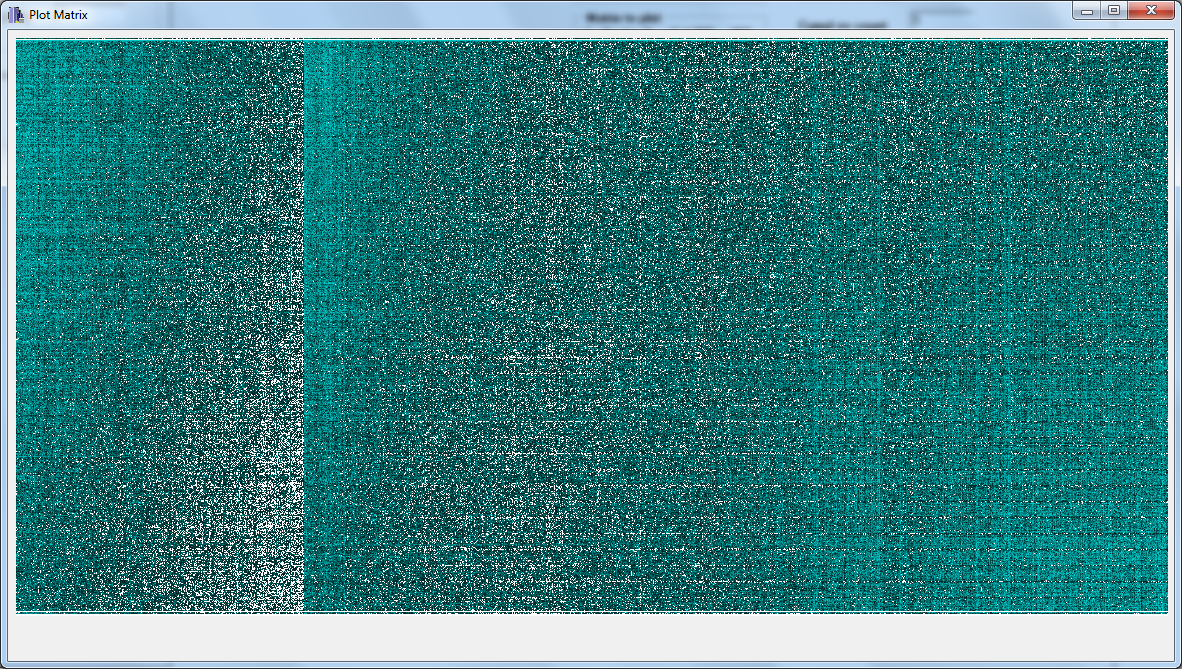
\includegraphics[width = \textwidth]{Pictures/labTests/discri_middle.png}
    \caption{Matrix response for the discriminators half activated.}
    \label{fig:homogeneityMi26}
  \end{figure}
  
  Afterward, the thresholds are set to the lowest and highest value to look for defect pixels in the matrix.
  On the one hand, few pixels can be always activated even if the discriminators were closed.
  The figure~\ref{fig:openPixel} depicts the matrix output for all the discriminators closed.
  Therefore, a line is always activated, as well as few pixels in a column and they are increasing the fake hit rate of the matrix.
  A solution exists to disconnect some discriminators in order to reduce the noise of defect columns thanks to the \gls{JTAG} program, nevertheless, no solution during the sensor programming exists to remove the defect lines.
  On the other hand, few pixels can be always deactivated even if the discriminators are completely opened, thus, they are not able to detect any physics signal.
  This behavior is represented on the figure~\ref{fig:closePixel} and no solution exists to make them working properly.
   
  \begin{figure}[!h]
    \centering
    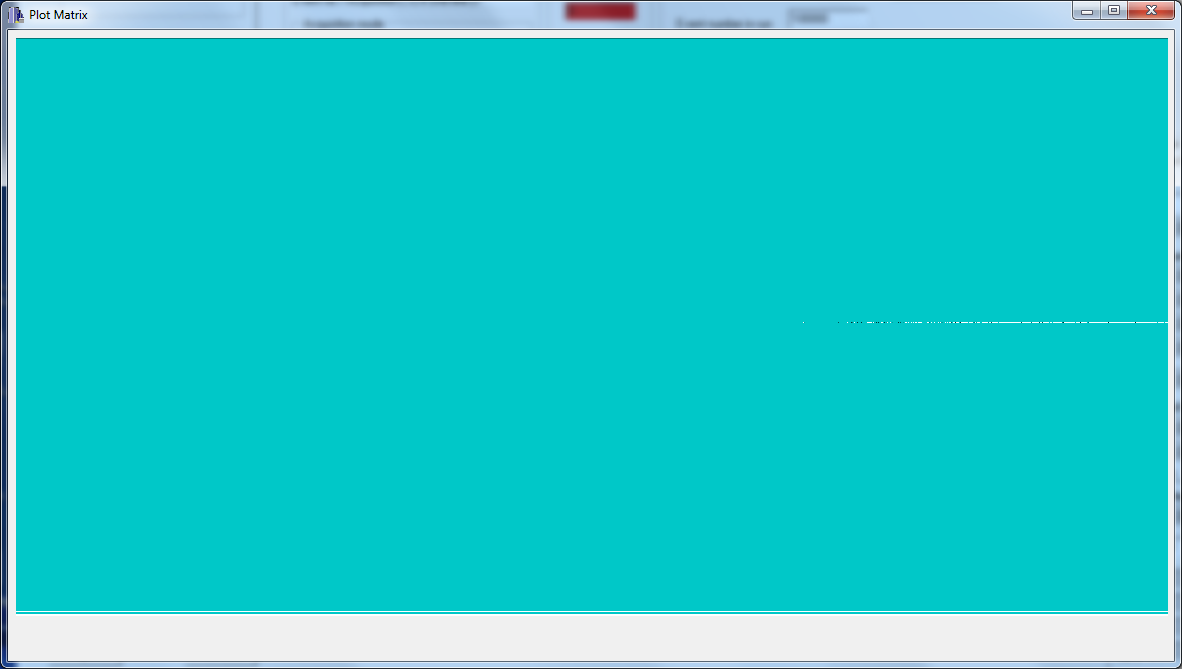
\includegraphics[width=\textwidth]{Pictures/labTests/th0.png}
    \caption{Matrix response in discriminator mode, where all the discriminators are opened. On the right of the matrix, one line is not working correctly and some pixels are never activated}
    \label{fig:openPixel}
  \end{figure}
   
  \begin{figure}[!h]
    \centering
    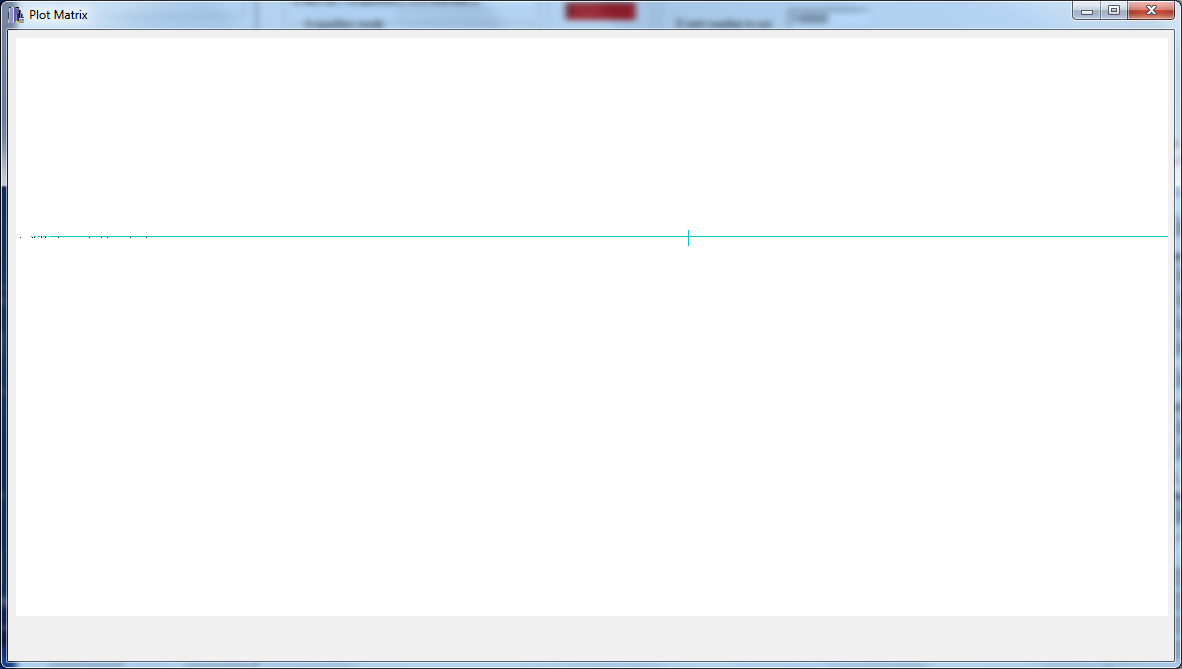
\includegraphics[width=\textwidth]{Pictures/labTests/th255.png}
    \caption{Matrix response in discriminator mode, where all the discriminators are closed. One line of pixels is always activated, as well as few pixels in the same column. This will increase the fake hit rate of the sensor.}
    \label{fig:closePixel}
  \end{figure}

  \subsection{Threshold scan}

  The noise performance of the sensor is determined through a threshold scan around the "middle-point" found before.
  This consists to record the normalise response of the discriminators or the discriminators and the pixels for different threshold values.
  For the first possibility, an external voltage is injected into the discriminators, while the matrix output is disconnected.
  Only the noise contribution coming from the discriminator is thus determined.
  In this work, the noise performance results presented were done without injected an external voltage, but rather with the sensitive system connected to the discriminators.
  Usually, 29 runs containing between 50 to 1000 are stored.
  The files created are used to firstly, build a configuration file containing the DAC values of each sub-matrix for the different thresholds applied.
  The threshold is here defined has the voltage applied to the discriminators.
  Afterward, this file is analysed and converted to create an output file containing a hit average picture of each sub-matrix for each step.
  Then, a macro based on C++ and ROOT framework is reading the hit average picture to plot the transfer function, also called "S" curve, as represented on the figure~\ref{fig:transfer}.
  It shows the normalised response of the 288 discriminators and the pixels contained in this sub-matrix as a function of the threshold applied in millivolts.
  The temporal noise of each pixel is calculated from the derivative of the "S" curve and is represented here in the left plot of the figure~\ref{fig:TN&FPN}.
  The mean value of the distribution obtained the mid-point threshold of a pixel.
  The dispersion of the mid-point threshold corresponds to the fixed pattern noise, represented on the right plot of the figure~\ref{fig:TN&FPN}.
  
  \begin{figure}[!h]
    \centering
    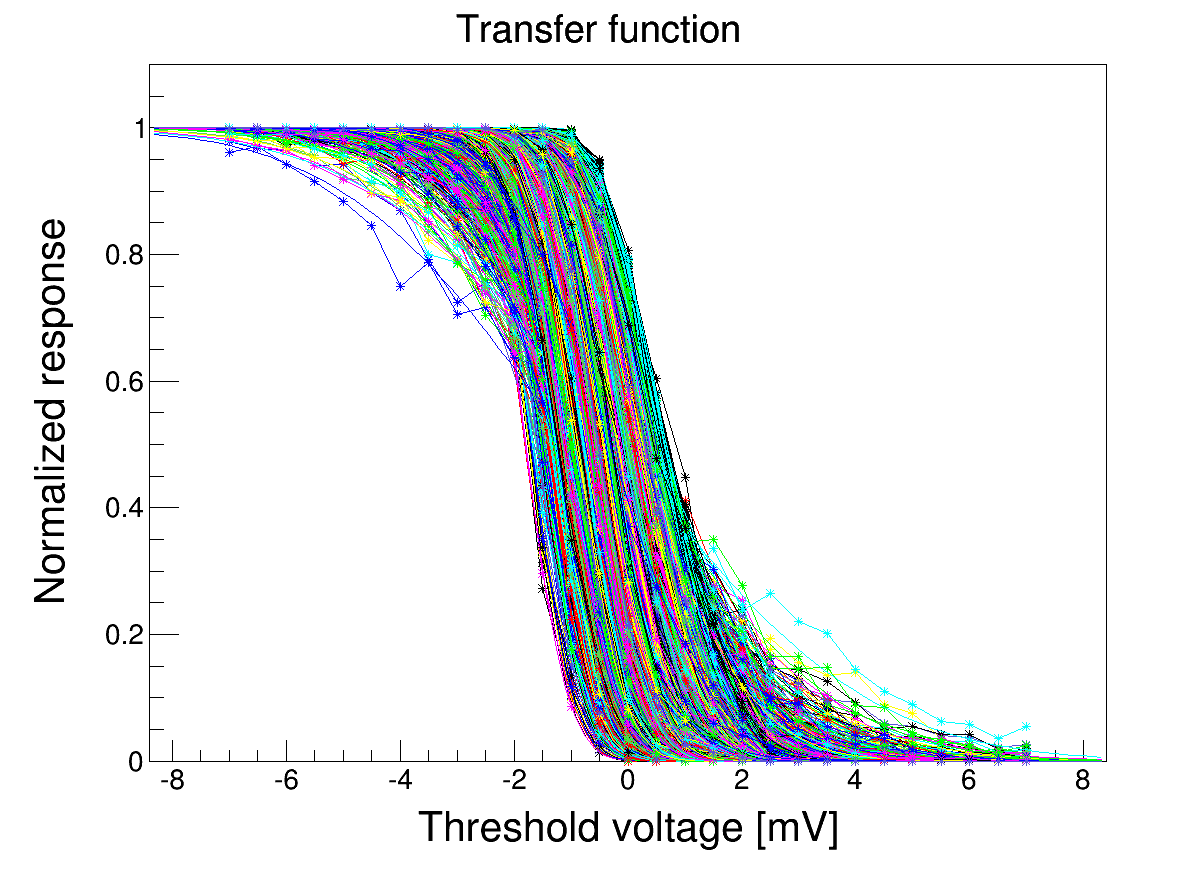
\includegraphics[width=0.7\textwidth]{Pictures/labTests/transfer_B.png}
    \caption{Pixels response of a threshold scan around the middle-point of discriminators for a sub-matrix.}
    \label{fig:transfer}
  \end{figure}

  \begin{figure}[!h]
    \centering
    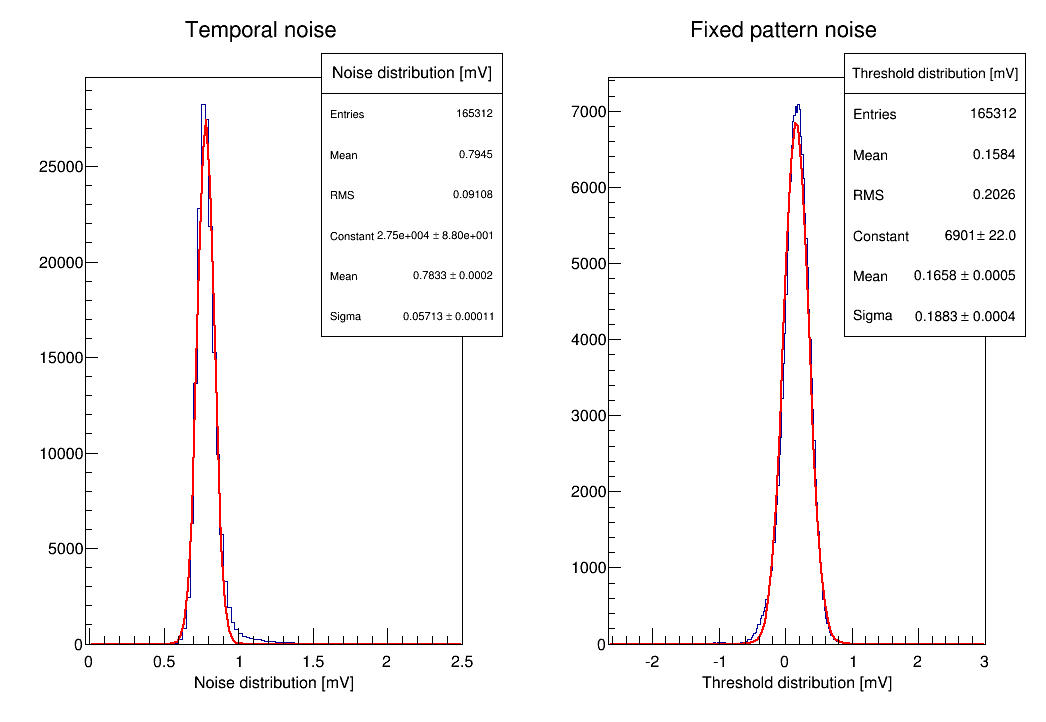
\includegraphics[width=0.8\textwidth]{Pictures/labTests/noise_A.png}
    \caption{Noise performances of a sub-matrix for the discriminators and the pixel array output. The temporal noise is plotted on the left plot, whereas the fixed pattern noise is represented on the right plot.} 
    \label{fig:TN&FPN}
  \end{figure}

  The plot on the left in figure~\ref{fig;TN&FPN} represents the temporal noise, while the right one represents the fixed pattern noise.
  The systematic offset of the discriminator is extracted from this measurements (the mean value of the temporal noise, the mean value and the sigma value of the fixed pattern noise).
  To calculate the discriminator thresholds of each sub-matrix for a given \gls{SNR}, the total noise is determined as:
  
  \begin{equation}
    \rm{Total~noise} = \sqrt{<\rm{TN}>^2 + <\rm{FPN}>^2}
  \end{equation}

  For a given S/N cut $\sigma$, the thresholds are determined by:

  \begin{equation}
    \rm{Threshold~(mV)} = \rm{Total~Noise} \times \sigma + \rm{offset}
  \end{equation}

  This is converted into the DAC values by taking into account the DAC offset and the DAC slope, which is assumed to be $0.25~\rm{mV}$:
  
  \begin{equation}
    \rm{Threshold~(DAC)} = \frac{\rm{Threshold~(mV)} - \rm{DAC}_{\rm{offset}}}{\rm{DAC}_{\rm{slope}}}
  \end{equation}



  \subsection{Noise measurements}

  Once the thresholds are defined for the different cuts, the fake hit rate of the matrix, as well as the detection homogeneity is determined.
  A quick step consists of using the DAQ software and acquiring ten-thousands events in the dark to determine the noise qualitatively. 
  The fake hit rate per event per pixel is then considered as:

  \begin{equation}
    \rm{F.H.R} = \frac{\rm{Number~of~hits}}{\rm{Number~of~events} \times \rm{Number~of~pixels}} 
  \end{equation}
  
  The figure~\ref{fig:darkEvents} is representing the accumulation in the dark of ten thousand events for a threshold five times bigger than the noise.
  The measured fake hit rate was below $10^{-4}~\rm{hits/pixel/events}$.

   \begin{figure}[!h]
    \centering
    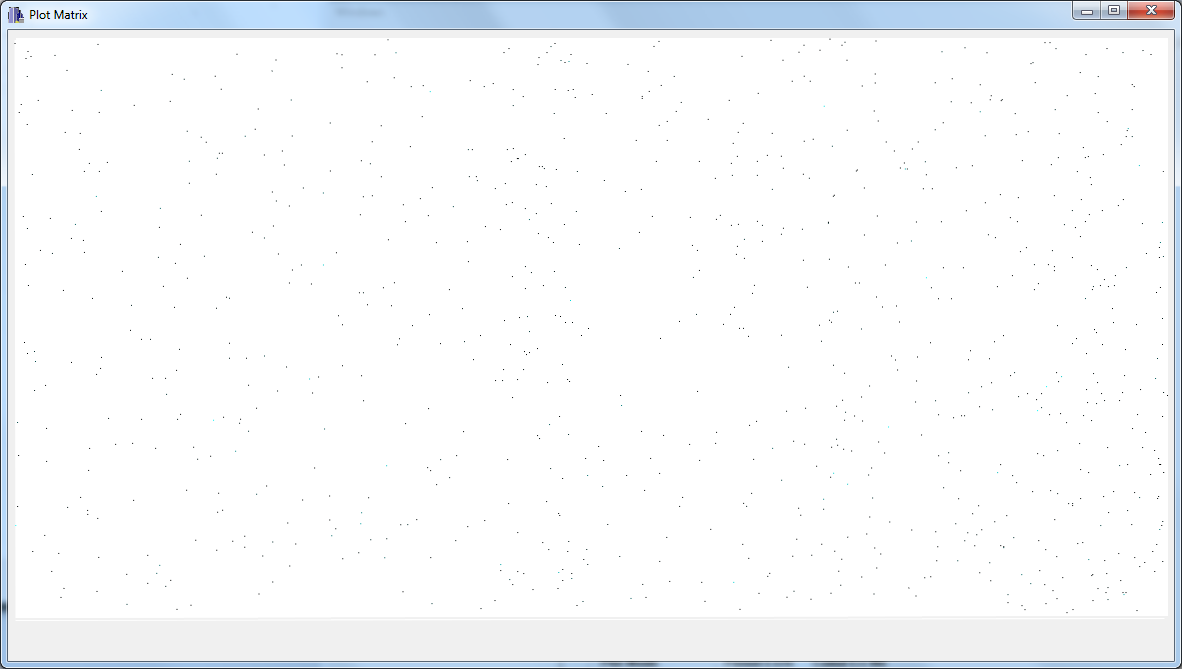
\includegraphics[width=0.6\textwidth]{Pictures/labTests/dark_10kEvents_not_noisy.png}
    \caption{Accumulation of 10k events at a thresholds of 5 times the noise acquired in the dark.}
    \label{fig:darkEvents}
  \end{figure}

  Then, an iron 55 source is used to control the homogeneity of the thresholds determined before.
  The figure~\ref{fig:fe55} represents the accumulation of ten thousand events for a threshold five time bigger than the noise with an iron source on top of the sensor.
  
  \begin{figure}[!h]
    \centering
    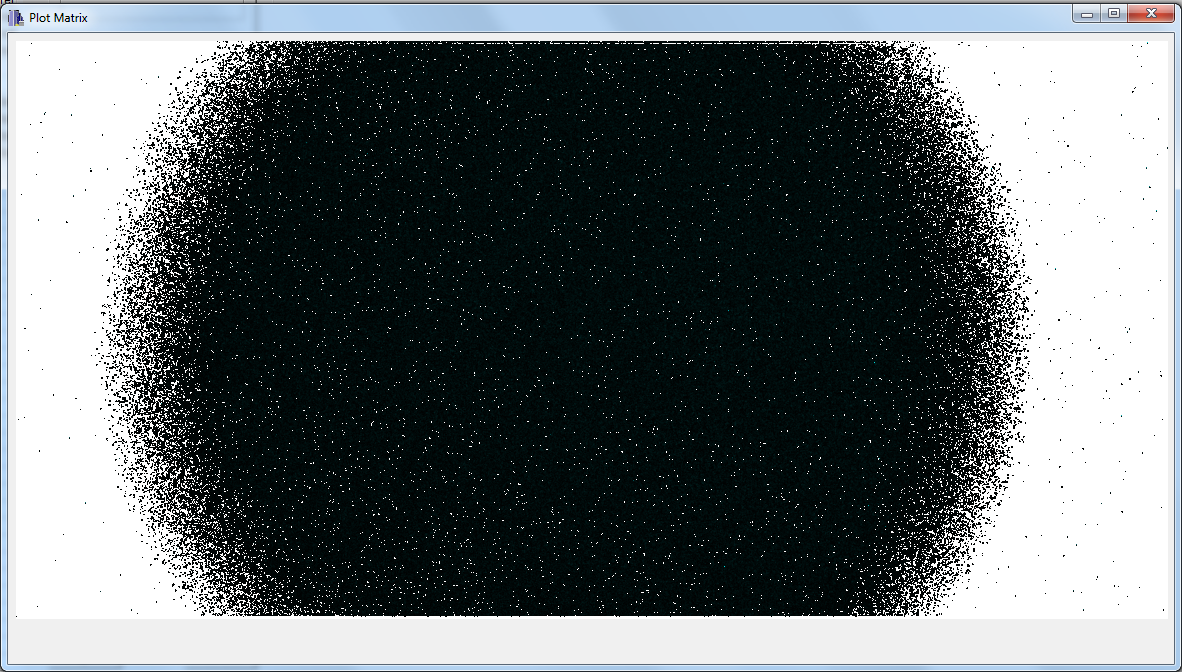
\includegraphics[width=0.6\textwidth]{Pictures/labTests/10kEvents_Fe55_cut5sigma.png}
    \caption{Accumulation of 10k events at a thresholds of 5 times the noise with $^{55}\rm{Fe}$ radiation source.}
    \label{fig:fe55}
  \end{figure}

  Finally, in order to validate the sensor, the acquisition system used during the test beam is used to calculate quantitatively the fake hit rate.
  The auxiliary board is connected to a  Flex RIO board instead of the digital card.
  The test beam DAQ software developed by the IPHC is using a LabVIEW interface for the run control.
  It provides several useful information, such as the number of events acquired, the \textit{header}, the \textit{trailer} and the \textit{frame counter} of the sensor.
  This helps the user to know if the acquisition is running properly.
  If the \textit{frame counter} is different for each sensor, this points out a loss of synchronisation during the acquisition.
  Also, a different \textit{header} or \textit{trailer} such as the ones set in the JTAG software might point out a wrong connection.
  A second software is used to store the data into three files: a parameter file containing the run number, the event number, an index file and a binary file containing the raw data.
  Two acquisition modes are available. 
  The first one, used in test beam, acquires data only when a trigger is sent.
  The second one, stores all frames regardless the trigger status. 
  This acquisition is the one used in the lab, as only the noise of the sensor is measured.
   
  Several runs containing each one million events are acquired for different thresholds. 
  The data stored are analysed with a software developed by the IPHC and is called \gls{TAF}\cite{TAF2015}.
  It is based on C++ and the ROOT framework.
  The software reads the information of the hit pixels, reconstructs the clusters of hit pixels and in the case of a test beam is able to reconstruct tracks from the hit information.

  A method is used to determine the fake hit rate with respect to the number of pixels hit per event.
  From the distribution shown on the figure~\ref{fig:pixel/event}, which represents the number of pixels fired per event, the average fake hit rate is calculated as the mean of this distribution divided by the total number of pixels contained in the matrix.
    \begin{figure}
    \centering
    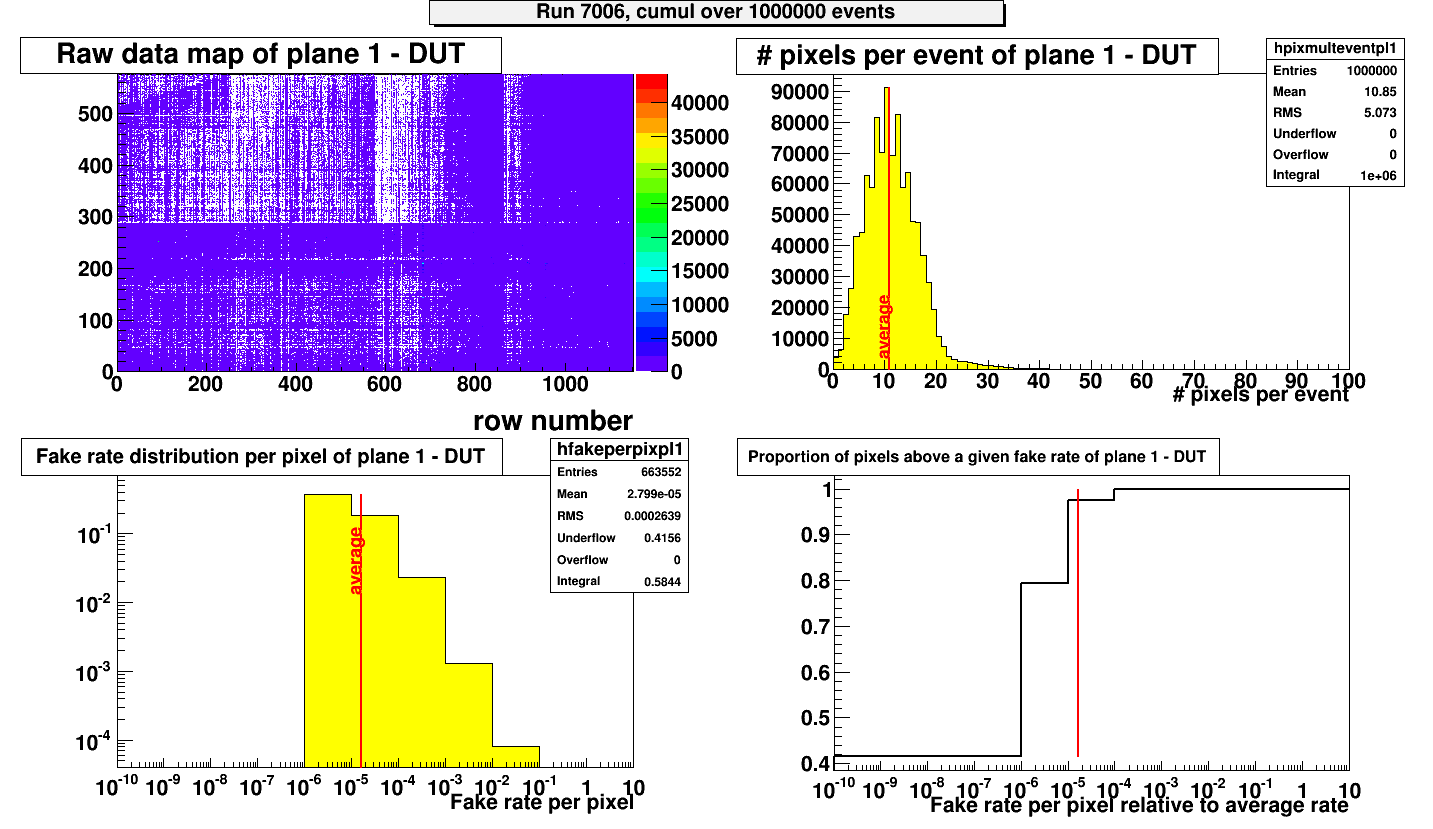
\includegraphics[width = \textwidth]{Pictures/labTests/FHR_AS01_chip3.png}
    \caption{Results of the fake hit rate measurement for a threshold three times bigger than the noise. The top left plot represents a raw picture of the million events accumulated over the whole matrix. The top right one is the distribution of the number of pixels hit per event. The bottom left plot is the fake hit rate per pixel distribution, while the bottom right one is the fake hit rate relative to the average rate distribution.}
    \label{fig:pixel/event}
  \end{figure}
  The error on the measurement is then the root mean squared of the distribution divided by the number of entries and the number of pixels inside the matrix.
  This calculation is done for different thresholds and the figure~\ref{fig:FHR} represents the average fake hit rate per pixel per event as a function of the threshold for one sensor of an aluminum module.
  The results are matching the expected behavior for a standalone MIMOSA-26 sensor as shown in figure~\ref{fig:mi26Perf}.

  \begin{figure}
    \centering
    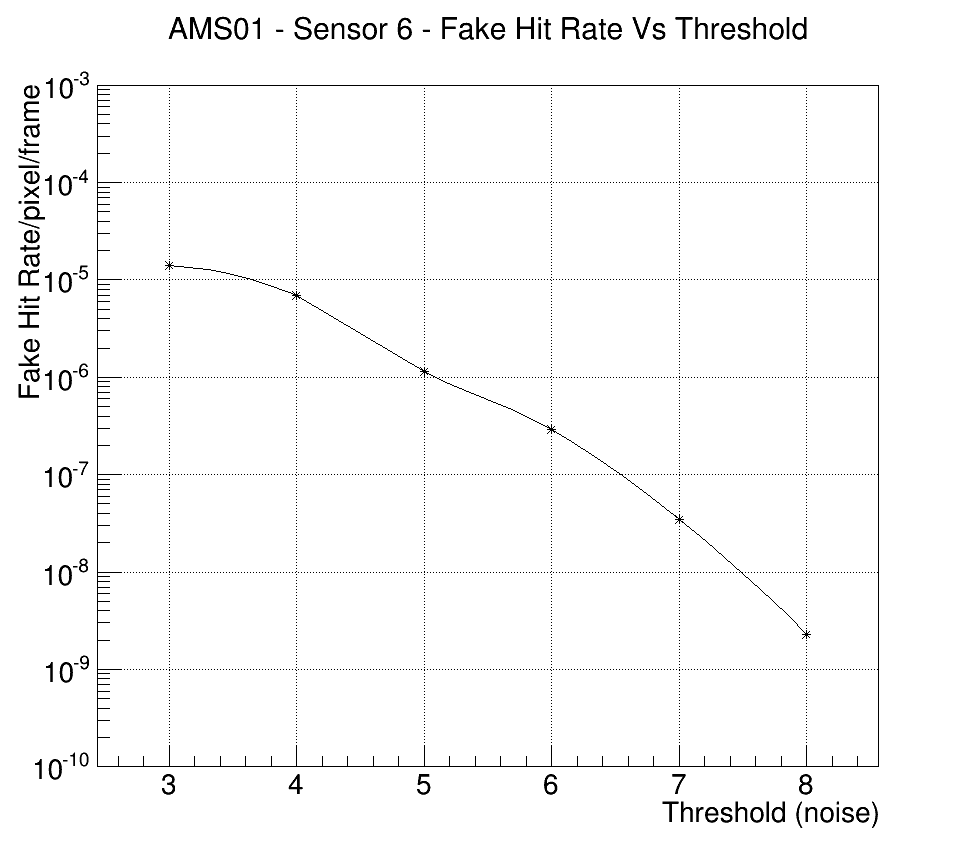
\includegraphics[width=0.7\textwidth]{Pictures/labTests/fake_sensor6.png}
    \caption{Distribution of the fake hit rate per pixel.}
    \label{fig:FHR}
  \end{figure}

\section{Conclusions}

  The assembly procedures and the tests performed in the laboratory were introduced along this chapter.
  Only the results for one sensor were presented.
  Nonetheless, all the modules have a same behavior as the one expected for one single MIMOSA-26.
  So far, for the new PLUME versions which have a narrower flex-cable and which should embed only $0.35~\%$ of the radiation length, different prototypes were built. 
  The first ladder using copper module was assembled in January 2016.
  New ladders are currently being built and the collaboration is expecting to test them in the DESY test beam facility in November.
  Nevertheless, the aluminum ladder seems to be more challenging to build.
  Indeed, the three first mirrored versions produced have a connector problem, that could have been damaged by plugging and unplugging the jumper cable.
  This problem did not occur with the copper mirrored versions and this might come from a more fragile flex-cable.
  Ideally, each module should have is own jumper cable and this should not be disconnected.
  Nevertheless, for shipping them, there is no other solution.
  The collaboration is thinking of a tool which will reduce the stress applied to the connector.

  The next chapter deals with the tests performed in real condition at the CERN-SPS facility with the PLUME-V1 prototype in 2011.


